\documentclass[german]{report}
\usepackage[ngerman]{babel}
\usepackage[ansinew]{inputenc}
\usepackage{graphicx}
\usepackage{here}
\usepackage{pdfpages}
\usepackage{url}
\usepackage{amssymb,amsmath}
\usepackage{listings}
\usepackage{multirow}
\usepackage{fancyhdr}
\usepackage{lmodern}

\usepackage{color}
\usepackage{xcolor}
\usepackage{listings}

\usepackage{caption}
\DeclareCaptionFont{white}{\color{white}}
\DeclareCaptionFormat{listing}{\colorbox{gray}{\parbox{\textwidth}{#1#2#3}}}
\captionsetup[lstlisting]{format=listing,labelfont=white,textfont=white}



  \RequirePackage{draftwatermark}
  \SetWatermarkText{DRAFT}

\begin{document}

\pagestyle{fancy}
\lhead{\color{red}\textbf{DRAFT}}
\chead{- Knowledge Based Systems - }
\rhead{\includegraphics*[width=2.0cm]{abbildungen/dhbwlogo.png}}

\cfoot{Christoph Schabert, Stephan Alaniz, Jan Brodhacker (TINF11-AI\/BC) \\DHBW Mannheim}
\lfoot{\color{red}\textbf{DRAFT}}
\rfoot{\thepage}
\fancyhfoffset{\marginparsep}
\renewcommand{\footrulewidth}{1.0pt}
\renewcommand{\headrulewidth}{1.0pt}
\renewcommand{\headheight}{30pt}
\pagenumbering{arabic}





\begin{titlepage}

\begin{flushright}
    \includegraphics*[width=4.0cm]{abbildungen/dhbwlogo} \\ 
\end{flushright}
\begin{center}
\vspace{1.5cm}
\Huge{ \textsf{Knowledge Based Systems}} \\
	Yavalath\\
    \vspace{4cm}
 \normalsize{
    \begin{tabular}{ll}
    	Names: & {Schabert Christoph  Alaniz Stephan  Brodhacker Jan} \\
    	Course: & {TINF-AI11/BC}	\\
    	Lecturer: &  HR. Dr. Dr. Dr. Dr. Vossen\\
    	working period: & 09.09.2013 bis XX.XX.2014
    \end{tabular}\\
    }
\end{center}

\end{titlepage}

\newpage
\section*{Statutory declaration}\thispagestyle{empty}
I herewith declare that I have completed the present thesis independently making use only of the specified literature and aids. Sentences or parts of sentences quoted literally are marked as quotations; identification of other references with regard to the statement and scope of the work is quoted. The thesis in this form or in any other form has not been submitted to an examination body and has not been published.\\
\\
Stephan Alaniz:\\
Heidelberg, the \_\_.\_\_.2013 \hspace{2.5cm} .............................. \\
\hspace*{6.5cm} (signature)\\
\\
Christoph Schabert:\\
Heidelberg, the \_\_.\_\_.2013 \hspace{2.5cm} .............................. \\
\hspace*{6.5cm} (signature)\\
\\
Jan Brodhacker:\\
Heidelberg, the \_\_.\_\_.2013 \hspace{2.5cm} .............................. \\
\hspace*{6.5cm} (signature)\\

\newpage
\setcounter{page}{1}



\tableofcontents

\listoffigures

\renewcommand{\lstlistlistingname}{Verzeichnis der Quellcodes}
\renewcommand{\lstlistingname}{Quellcode}
\lstlistoflistings

\bibliographystyle{plain}
\bibliography{Quellen}

\newpage

\chapter{Intruduction}
\label{sec:chapter1}
\section{Goal and Motivation}
The goal of this project is to implement a game called Yavalath. And to develop
two different Artificial Intelligences, which are able to play the game and win
against nearly every human player.

\section{Technical Notes}
The implementation of the game and the ai-players with a fully functional
graphical user interface is availible on GitHub und the the following url:
\begin{quotation}
    https://github.com/belafarinrod91/KBSYavalath (hep: 25.10.2013)
\end{quotation}
This project is under no license or otherwise protected, feel free to clone the
Git repositry and compile it yourself.


This publication was written in \LaTeX an compiled with MikeTex.

\chapter{The Game - Yavalath}
\label{sec:chapter2}
In this chapter the history of Yavalath, and the game is explained.
% #TODO: tech more!!!
\section{History}
Yavalath is the most successgul game evolved by LUDI in 2007 and published in 2009 by Nestorgames (Spain). LUDI is a game-generating computer program 
that implements an algorithm for generating new games. This LUDI software system not only defines the scope and rules of the game, it also interpets 
the game and coordinates testplays to measures the game quality.
LUDI was developed by Cameron Browne as part of his PhD in AI and game design,
also was he awarded with the Dean's Award for Outstanding Thesis
\cite{EvolutionGameDesign}. \\

In 2011 Yavalath was ranked onto place 99 from the BoardGameGeek
community\footnote{\url{www.boardgamegeek.com}} out of 4300 abstract games ever invented.
It was also rated onto place 8 out of 200 abstract games invented in 2007. \\

Yavalath won 2012 the Humies Award for Human-Competitive Result Produced by Genetic and Evolutionarty Computation

\section{Categorisation}
Yavalath is a mixture of connect and patter building game. The BoardGameGeek
community categorised Yavalath as a abstract game because it was the first
computer-generated game with such a huge success.

Also Yavalath inspired a new game categorie thats called:
\begin{quote}
	winning with a line of N and losing with a line of N-1.
\end{quote}

The name Yavalath was randomly created by a Markovian algorithm.

\section{The Rules}
The Rules for Yavalath are pretty simple, what makes it easy to learn. But its
still novel so that the game is still intressting. 
One of the reasons why the game became so successfull is that Yavalath achieves
a good balance between simplysiti and a kind of innovation.

Yavalath is for two or three players and the average playingtime per game is 10 minutes\footnote{this was voted by the BoardGameGeek comunity, source:\url{http://boardgamegeek.com/boardgame/33767/yavalath}}.

The board is a hexagon with 5 spaces on every side, that is initally empty.
With that specifications there are 61 free cells in total, as to see in Illustration \ref{fig:yav_board}.

\begin{figure}[ht]
\centering
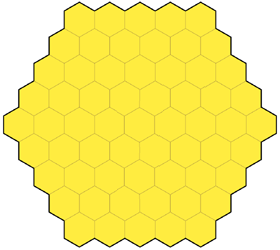
\includegraphics[width=0.95\textwidth]{Abbildungen/yav_emptyBoard.png}
\caption[The Yavalath game board, Source:\cite{yvalathHP}]{The Yavalath game board}
\label{fig:yav_board}
\end{figure}


Every turn a players place a pieces of their colour onto the board. 

This goes on untill:
\begin{itemize}
	\item on player have won
	\item all but one players have lost
	\item all cells are filled and it is a draw
\end{itemize}

As Soon as a Player formes a line of three pices in a row the player looses.

A player can win with two different methods:
\begin{enumerate}
	\item one players manage to make a line of four or more pices of his color (In illustartion  \ref{fig:yav_4inarow} the white player won).
	\item one player forece another player to form a line of three pices what is called a forced move. (In illustartion  \ref{fig:yav_forceMove} the black player is forced to move to prevent the white player from winning. in).
\end{enumerate}

\begin{figure}[ht]
\centering
\includegraphics[width=0.95\textwidth]{Abbildungen/yav_4inarow.png}
\caption[Four in a row wining, Source:\cite{yvalathHP}]{Four in a row wining}
\label{fig:yav_4inarow}
\end{figure}


\begin{figure}[ht]
\centering
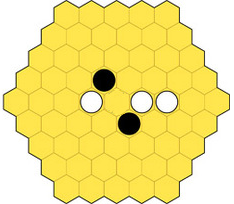
\includegraphics[width=0.95\textwidth]{Abbildungen/yav_forceMove.png}
\caption[Forced move winning, Source:\cite{yvalathHP}]{Forced move winning}
\label{fig:yav_forceMove}
\end{figure}


This leads to a so called Rule Tension, in this case four is a row is good but three in a row is bad. This means the Player cant just extend lines and must think about the pros and cons of every move he makes.\cite{yvalath}

\section{Tactics and Strategy}
Cameron Browne himsself defined some taktics and strategies and described them in his publication. He started to describes a number of chooices for the first move and a number of patterns that have a good chance of winning.


The first move is crucial for the folowing tactics and for the chance to win.
In Illustration \ref{fig:yav_winChance} is shown a Yavalath board with the win chance for the first move, the bigger the bouble the bigger the win chance. As its good visable that a centerd first move has the biggest win chance.\cite{yvalathHP}


\begin{figure}[ht]
\centering
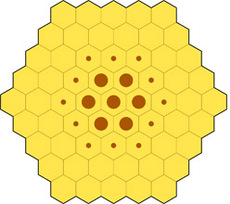
\includegraphics[width=0.95\textwidth]{Abbildungen/yav_winChance.png}
\caption[The win chance for the first Move, Source:\cite{yvalathHP}]{The win chance for the first Move}
\label{fig:yav_winChance}
\end{figure}


An other good chooice for a first move is to start with a pattern. The Triangle starting pattern is an excelent example for a first move pattern (the Triangle starting pattern is shwon in illustration \ref{fig:yav_triangle}) on the left side). because it provides a huge number of chances to win by a forced move. Also its hard to stop a player that used the triangle pattern as a starting move. The only way to stop it is to forsee it pretty early and prevent the player from forming the triangle.
On the right side of illustration \ref{fig:yav_triangle} a possible outcome of the triangle starting possition where the black player has losst by a forced move.\cite{yvalathHP}

\begin{figure}[ht]
\centering
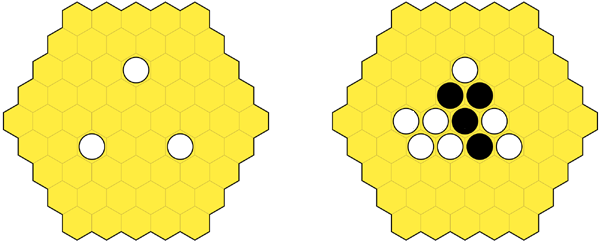
\includegraphics[width=0.95\textwidth]{Abbildungen/yav_triangle.png}
\caption[The triangle starting pattern, Source:\cite{yvalathHP}]{The triangle starting pattern}
\label{fig:yav_triangle}
\end{figure}

In Yavalath a Triangle is always a good pattern, for example the small triangle (as seen in illustration \ref{fig:yav_smallTriangle}). The Reason that the small triangle is such a strong pattern is because it can foram a huge number of winning chances. 


\begin{figure}[ht]
\centering
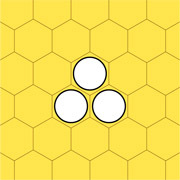
\includegraphics[width=0.45\textwidth]{Abbildungen/yav_smallTriangle.png}
\caption[A small triangle pattern, Source:\cite{yvalathBGG}]{A small triangle pattern}
\label{fig:yav_smallTriangle}
\end{figure}

To show that the small triangle is a good pattern two winning patterns are shown in illustration \ref{fig:yav_smallTriangleWin1} and in illustration \ref{fig:yav_smallTriangleWin2}. Both force the black player to loose by a force move. Also its possible to turn a pattern by 120� Degree, with that in mind there are at least six possible winning situations. If a opponent player try to form a triangle its recommendet to stop him as soon es possible.\cite{yvalathBGG}



\begin{figure}[ht]
\centering
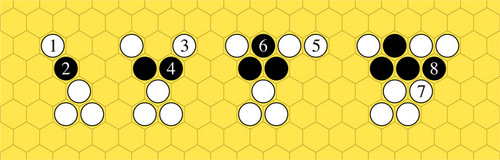
\includegraphics[width=0.95\textwidth]{Abbildungen/yav_smallTriangleWin1.png}
\caption[A small triangle winning pattern, Source:\cite{yvalathBGG}]{A small triangle winning pattern}
\label{fig:yav_smallTriangleWin1}
\end{figure}

\begin{figure}[ht]
\centering
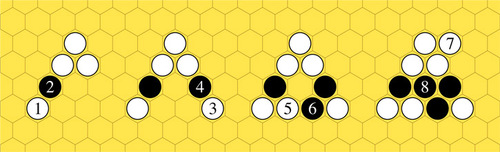
\includegraphics[width=0.95\textwidth]{Abbildungen/yav_smallTriangleWin2.png}
\caption[A second small triangle winning pattern, Source:\cite{yvalathBGG}]{A second small triangle winning pattern}
\label{fig:yav_smallTriangleWin2}
\end{figure}


\chapter{Technical Implementation}
\label{sec:technImplementation}
The game was implemented in Java, a platform-independent programming language.
It offers many extensions to develop such a complex game. Java is also fast
enough to calculate all dependecies and to return the user a
response on their interaction with the game in a suitable time. But therefore
isn't a high-end computer needed. In this context no frameworks were used. The
graphical user interface was realized with the assistance of the GUI-Library
SWING for Java, which is based on the Abstract-Window-Toolkit (AWT).  




\chapter{Artificial Intelligences}
\label{sec:artificIntelligences}
All in all this implementation of Yavalath shows two approaches of an artificial
intelligence. On the one hand there is the so called UTCAI
\footnote{UCT : http://senseis.xmp.net/?UCT}, which can has three different
levels of difficulty. And the other hand there is the simple approach of a
random AI. Both approaches are explained in a more detailed view in the next two
sections. 


\section{Random-AI}
The Random-AI is one of the two implemented Artificial-Intelligences and is the
more easier opponent for the player. Actually the Random-AI is definitely the
easier technical-implementation of the both implemented AIs.

\begin{lstlisting}[label=some-code,caption=Some Code]
public void here() {
	goes().the().code()
}
\end{lstlisting}

% #TODO: Tech the Dokument



\end{document}
